\documentclass{article}
\usepackage{amsmath, fullpage}
\usepackage[portuguese]{babel}
\usepackage{graphicx}
\usepackage{color}
\usepackage[normalem]{ulem}
\newcommand{\uvec}[1]{\boldsymbol{\hat{\textit{#1}}}}
\graphicspath{{image/}}
\begin{document}

\title{Introdução à mecanica dos fluidos \\ Fenômenos de transporte}

\author{Henrique Bernardes}
%\date{\vspace{-5ex}}
\maketitle
\thispagestyle{empty}

\section{Início}
Começamos com a ideia de um pequeno elemento estacionário de fluido em uma certa posição arbitrária de massa do fluido como visto em \ref{fig:forcasuperficieecampo}. Também, sabemos que existem dois tipos de forças que atuam sobre esse elemento:
\begin{itemize}
     \item forças de superfície \( \rightarrow \) devidas à pressão
     \item força de campo \( \rightarrow \) igual ao peso do elemento(no caso estudado, igual a força gravitacional)
\end{itemize}

O peso \( \delta W\) (ou \( d\vec{F_g}\)) atua no sentido negativo da direção z e pode ser descrito como:
 \begin{equation}
      \delta W = \vec{g}*dM 
 \end{equation}
mas como sabemos da fórmula de massa específica, \( dM = \rho dV \), onde \( dV= dxdydz\), a equação se torna:
\begin{equation}
     \delta W = \vec{g} \rho  \delta x \delta y \delta z
\end{equation}
Por fim, \( \gamma = \rho \vec{g}\), assim,

\begin{equation}
     \delta W = \gamma  \delta x \delta y \delta z
\end{equation}


\begin{figure}[!h]
     \centering
     \def\svgwidth{0.4\textwidth}
     \input{image/inomeado.eps_tex}
     \caption{\label{fig:forcasuperficieecampo} Forças de superfície e campo atuando em um pequeno elemento de fluido.}
     \hfill
\end{figure}
 

Sabemos que a soma das forças sobre esse elemento de volume d\sout{V} deve ser 0 para atender à condição de equilíbrio, ou seja

\begin{equation}
     d\vec{F}=d\vec{F_g}+d\vec{F_p}
     \label{equacaoGeral}
\end{equation}

Já deduzimos que as forças de campo se resumem à:

\begin{equation}
     d\vec{F_g}=dM*\vec{g}=\rho \vec{g} dxdydz
\end{equation}

Agora, para as forças de superfície, temos o seguinte:

\begin{equation}
     d\vec{F_p}=P(x,y,z)A
\end{equation}

Considerando a componente x e expandindo em Taylor:
\begin{align*}
d\vec{F_{px}} &= [P(x,y,z)-P(x+dx,y,z)]dydz \rightarrow  P(x+dx,y,z)=P(x,y,z)+\frac{\partial P}{\partial x}dx+...\\ 
&= \left[P(x,y,z)-P(x,y,z)-\frac{\partial P}{\partial x}dx\right]dydz\\
&= -\frac{\partial P}{\partial x}dxdydz\ .
\end{align*}
Então: 
\begin{equation}
    d\vec{F_{px}}= -\frac{\partial P}{\partial x}dxdydz\ .
\end{equation}
Para os outros componentes:
\begin{align}
d\vec{F_{py}}= -\frac{\partial P}{\partial y}dxdydz \\    
d\vec{F_{pz}}= -\frac{\partial P}{\partial z}dxdydz \
\end{align}

Assim sendo, temos o o seguinte:

\begin{equation}
     \sum{d\vec{F_p}} = \underbrace{-\left(\frac{\partial P\uvec{i}}{\partial x} + \frac{\partial P\uvec{j}}{\partial y} + \frac{\partial P\uvec{k}}{\partial z}\right)}_{\vec{\nabla} P}dxdydz
\end{equation}
Onde $d\vec{F_p}$ é um campo vetorial de força associado ao campo escalar de pressão.

Ou seja:

\begin{equation}
     \sum{d\vec{F_p}}=-\vec{\nabla}Pdxdydz 
\end{equation}

Substituindo os valores de $d\vec{F_p}$ e $d\vec{F_g}$ na equação \ref{equacaoGeral}, obtemos:

\begin{align*}
&d\vec{F_g} + d\vec{F_p}=0\\
&\rho \vec{g}dxdydz - \vec{\nabla}Pdxdydz=0\\
&(-\vec{\nabla}P + \rho\vec{g}) dxdydz=0\\
&(\underbrace{-\vec{\nabla}P}_a + \underbrace{\rho\vec{g}}_b)=0\
\end{align*}
O termo \textit{a} indica a força de pressão resultante por unidade de volume em um ponto. Já o termo \textit{b} indica a força de campo por unidade de volume em um ponto.
\newpage
Decompondo nas direções x, y, e z:

\begin{align}
-\frac{\partial P}{\partial x} + \rho \vec{g}=&0\\
-\frac{\partial P}{\partial y} + \rho \vec{g}=&0\\
-\frac{\partial P}{\partial z} + \rho \vec{g}=&0\
\end{align}

Escolhendo o eixo z para cima:
\begin{figure}[!h]
     \centering
     \def\svgwidth{0.25\textwidth}
     \input{image/gCord.eps_tex}
     \caption{\label{fig:gravidadeCoordenadas} Eixo de coordenadas com vetor $\vec{g}$ indicado.}
     \hfill
\end{figure}

vemos então que:
\begin{align*}
\frac{\partial P}{\partial x}=0 ;\ 
\frac{\partial P}{\partial y}=0 ;\
\frac{\partial P}{\partial z} = -\rho \vec{g}\
\end{align*}

Assim sendo, como $P$ é uma função de uma só variável, a derivada parcial pode ser substituida pela derivada total:
\begin{equation}
     \frac{dP}{dz}=-\rho \vec{g}
     \label{equacaoFinalDerivada}
\end{equation}

Isto é, assumindo as seguintes premissas:
\begin{enumerate}
     \item O fluido é estatico;
     \item A gravidade é a única força de campo;
     \item O eixo z é vertical para cima.
\end{enumerate}

 
Para um líquido incompressível, $\gamma = cte$, ou seja, $\rho = cte$ e $g = cte$. Assim sendo, manipulando e integrando a equação \ref{equacaoFinalDerivada}, aplicando as condições de contorno, onde consideramos a pressão no nível de referência (z0) como sendo $P_0$, então a pressão P no nível z é dada por:

\begin{align*}
\frac{dP}{dz} &=-\rho g \\
dP &= -\rho g dz\\
\int_{P_0}^{P} \,dP &= -\rho g \int_{z_0}^{z}\,dz \\
P-P_0 &= -\rho g (z-z_0) \\
\end{align*}

\begin{equation}
\boxed{P-P_0 = +\rho g (z_0-z)}     
\label{eqFinal}
\end{equation}

Como visto na equação \ref{eqFinal}, a pressão em um líquido incompressível em repouso depende da altura h($h=z_0-z$) do fluido em relação a um plano de referência e \textbf{não} é influenciada pelo tamanho ou forma do tanque no qual o fluido se encontre. Também, a equação \ref{eqFinal} só é válida para fluidos na qual o peso específico $\gamma$ é constante. Para aqueles na qual $\gamma$ não é constante, a forma como varia deve ser especificada antes que a equação \ref{equacaoFinalDerivada} possa ser integrada.



\subsection{Exercicio 11.1}
Vamos calcular a pressão \textbf{manométrica}(ou seja, em relação à pressão atmosférica) na interface gasolina-água e na parte inferior do tanque em $\frac{lbf}{in^2}$ e a altura de carga da coluna de água em $ft$:
\begin{figure}[!h]
     \centering
     \def\svgwidth{0.5\textwidth}
     \input{image/exercicio11_1.eps_tex}
     \caption{\label{fig:exercicio11_1} Exercicio 11.1}
     \hfill
\end{figure}
Primeiro, calculamos a pressão no ponto 1, indo do ponto 0 ao ponto 1, tendo $\gamma_{gasolina}=42.5 \frac{lbf}{ft^3}$ e $\gamma_{agua}=62.4 \frac{lbf}{ft^3}$:

\begin{align*}
p_1 - p_0 &= \gamma_{gasolina}h_{1\rightarrow0}\\     
p_1 - p_0 &= \gamma_{gasolina}h_{1\rightarrow0}\\
p_1 - p_0 &= 42.5 \frac{lbf}{ft^3} * 17ft \\ 
p_1 - p_0 &= 722.5 \frac{lbf}{ft^2} \left|\frac{1ft^2}{144 in^2} \right| \\
p_1 - p_0 &= 5.02 \frac{lbf}{in^2}\\
\end{align*}

Tendo o valor da pressão no ponto intermediario em relação ao ponto 0, podemos calcular a pressão no ponto 2 com relação ao ponto 1(indo do ponto 1 ao ponto 2):

\begin{align*}
p_2 - p_1 &= \gamma_{agua}h_{2\rightarrow1} \\
p_2 &= \gamma_{agua}h_{2\rightarrow1} + p_1\\
p_2 &= 62.4 \frac{lbf}{ft^3} * 3ft + 722.5 \frac{lbf}{ft^2} + p_0\\
p_2 - p_0 &= 909.7 \frac{lbf}{ft^2} \left| \frac{1ft^2}{144in^2} \right| \\
p_2 - p_0 &= 6.32 \frac{lbf}{in^2}\\
\end{align*}

Assim sendo, calculamos a altura de carga da coluna de água:
\begin{align*}
h_{0\rightarrow2}&=\frac{p_2-p_0}{\gamma_{agua}}\\
h_{0\rightarrow2}&=\frac{6.32 lbf/in^2}{62.4 lbf/ft^3}\\
h_{0\rightarrow2}&=\frac{0.10 ft^3}{in^2} \left| \frac{144in^2}{ft^2} \right|\\ 
h_{0\rightarrow2}&=14.58ft
\end{align*}

\subsection{Medições de pressão}

A pressão em um ponto interior de uma massa de fluido pode ser designada ou por \textbf{pressão absoluta} ou por \textbf{pressão manométrica}. A pressão absoluta é a medida em relação à pressão zero absoluta, enquanto a pressão manométrica é medida em relação à pressão atmosférica local.

Pressões absolutas são sempre positivas, mas a pressão manométrica pode ser ou positiva ou negativa, a depender se a pressão está abaixo ou acima da pressão atmosférica. Uma pressão manométrica negativa é também chamada de pressão de vácuo. Por exemplo, uma pressão absoluta de 10psi poderia ser representada como uma pressão manométrica de -4.7psi se a pressão atmosférica local fosse 14.7psi, ou então como 4.7 psi de sucção/vácuo. 

Para a maioria  das análises de mecânica dos fluidos é prática usual utilizar a pressão manométrica.

\subsection{Manômetros}
São dispositivos de medição de pressão que envolvem o uso de colunas de líquidos em tubos verticais ou inclinados. 
\subsubsection{Tubo Piezométrico}
Consiste em um tubo vertical, aberto na parte superior e fixado a um recipiente cuja pressão se deseja determinar.

\begin{figure}[!h]
     \centering
     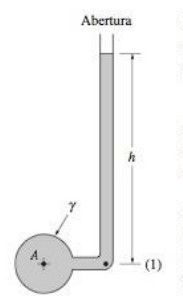
\includegraphics[width=0.2\textwidth]{tuboPiezometrico.jpg} 
     \caption{Tubo Piezometrico}
     \label{fig:tuboPiezometrico} 
     \hfill
\end{figure}

Uma vez que os manômetros envolvem colunas de fluidos em repouso, a equação fundamental que descreve seu uso é $p=\gamma h + p_0$, fornecendo a pressão em qualquer elevação no interior de um fluido homogêneo em termos da pressão de referência $p_0$ e da distância h entre $p$ e $p_0$. É importante mencionar que, uma vez que o tubo é aberto na parte superior, a pressão manométrica $p_0=0$, dado que:
\begin{align*}
p_{manometrica}&=p_{absoluta}-p_{atmosferica}\\
p_{manometrica}&=p_{atmosferica}-p_{atmosferica}\\
p_{manometrica}&=0
\end{align*}

Logo, a equação fundamental se reduz à:
\begin{align*}
     p = p_A = \gamma h 
\end{align*}

Embora o tubo piezométrico seja simples e preciso, apresenta algumas desvantagens:
\begin{enumerate}
     \item Só é apropriado se a pressão no recipiente for maior do que a pressão atmosférica(caso contrário, o ar seria sugado pelo sistema.);
     \item Só é apropriado se a pressão a ser medida for relativamente baixo, de modo que a altura necessária da coluna não seja muito elevada;
     \item O fluido no interior do recipiente cuja pressão deverá ser medida deverá ser um líquido e não um gás.
\end{enumerate}

\subsubsection{Manômetro de tubo em U}
Visando superar as dificuldades observadas no tubo piezométrico, utiliza-se o manômetro de tubo em U. O fluido no manômetro é chamado de \textbf{fluido manométrico}. Para determinar a pressão $p_A$ em termos das variações das alturas das colunas, começamos em uma extremidade do sistema e seguimos até a outra extremidade, utilizando apenas a equação fundamental.

\begin{figure}[h]
     \centering
     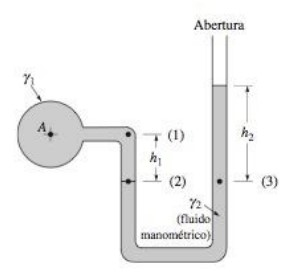
\includegraphics[width=0.3\textwidth]{manometroemtubosimples.jpg} 
     \caption{Manômetro em U simples} 
     \label{fig:manometroemtubosimples} 
     \hfill
\end{figure}



No caso da figura \ref{fig:manometroemtubosimples}, começamos na extremidade aberta seguindo para o ponto A($p-p_0 \rightarrow p_A-0$)\footnote{Vale a explicação mais detalhada: inicialmente, temos $p-p_0 = \gamma h$, onde $p$ é a pressão final e $p_0$ é a pressão inicial. Assim sendo, para determinar a diferença de pressão entre o ponto A e o ponto B, começamos no ponto A and terminamos no ponto B, ou seja, $p_B - p_A$. Poderiamos, alternativamente, determinar a diferença de pressão entre o ponto B e o ponto A, começando no ponto B e terminando no ponto A, ou seja, $p_A - p_B$. Segue a recomendação de \textbf{SEMPRE} seguir o caminho \textbf{ATÉ} o ponto onde se deseja conhecer a pressão. Logo, na figura \ref{fig:manometroemtubosimples}, começamos no ponto aberto e vamos para o ponto A, a equação se torna, então, $p_A-p_0$. Já na figura \ref{fig:manometroemtubodiferencial}, independe a ordem, mas, como indicado pela forma como foi fornecida a equação final no livro, devemos ir do ponto B até o ponto A, ou seja, $p_A - p_B$.} A pressão no ponto A e (1) são as mesmas e à medida que vamos do ponto (1) para o (2) a pressão aumentará em $\gamma_1 h_1$. A pressão no ponto (2) é igual à pressão no ponto 3, uma vez que as pressões em elevações iguais em uma massa contínua de fluido em repouso devem ser as mesmas(observe que não é possível "pular" do ponto (1) para um ponto de mesma elevação ao outro lado do tupo pois podem ser pontos de massa contínua de fluido diferentes). Com a pressão em (3) especificada, movemos para a extremidade aberta onde a pressão manométrica é 0. Como nos movemos para cima, a pressão decresce em magnitude $\gamma_2 h_2$. Em forma de equação:
\begin{align*}
\boxed{p_1-p_0 = p_A = \gamma_2 h_2 - \gamma_1 h_1}
\end{align*}

Uma das vantagens do manômetro de tubo em U está no fato que o fluido manométrico pode ser diferente do fluido no recipiente cuja pressão deve ser determinada. Por exemplo, o fluido em (A), (ainda na figura \ref{fig:manometroemtubosimples}) pode ser um líquido ou um gás. Se A contiver um gás, a contribuição da coluna de gás $\gamma_1 h_1$ é quase sempre desprezível de modo que $p_A=p_2$, ou seja, 
\begin{align*}
p_A=\gamma_2 h_2
\end{align*}

O peso específico $\gamma$, de um líquido, como fluido manométrico, é frequentemente representado em termos da densidade $D$, pela razão:

\begin{align}
     \gamma = D\gamma_{agua} = Dg\rho_{agua}
\end{align}
Um manômetro em U pode também ser utilizado para determinar a diferença na pressão entre dois recipientes, como na figura \ref{fig:manometroemtubodiferencial}

\begin{figure}[!h]
     \centering 
     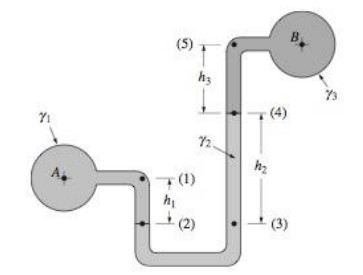
\includegraphics[width=0.3\textwidth]{manometroemtubodiferencial.jpg} 
     \caption{Manômetro em U diferencial} 
     \label{fig:manometroemtubodiferencial} 
\end{figure}
Para determinar diferença na pressão entre A e B começamos novamente em uma extremidade do sistema e seguimos até a outra.

A pressão em A($p_A$) é igual à pressão em (1), ou seja, $p_A = p_1$ e, a medida que nos deslocamos para o ponto (2), a pressão aumenta em $\gamma_1 h_1$. A pressão em (2) é igual à pressão em (3), ou seja $p_2 = p_3$ e, a medida que nos deslocamos para (4), a pressão diminui em $\gamma_2 h_2$. De forma similar, a medida que nos deslocamos de (4) para (5), a pressão diminui em $\gamma_3 h_3$. Por fim, temos que a pressão em (B) é igual à pressão em (5), ou seja, $p_B=p_3$. Em forma de equação:
\begin{align*}
\boxed{p_A-p_B=\gamma_3 h_3 + \gamma_2 h_2 - \gamma_1 h_1}
\end{align*}
\newpage
\subsection{Exercício 11.8} 

\begin{figure}[!h]
     \centering
     \def\svgwidth{0.8\textwidth}
     \input{image/exercicio11_8.eps_tex}
     \caption{\label{fig:exercicio11.8} Exercicio 11.8}
     \hfill
\end{figure}

Neste exercício, devemos determinar algumas coisas:
\begin{enumerate}
     \item A altura h
     \item A pressão manométrica na superfício AB
     \item A pressão absoluta do ar no topo do tanque se a pressão atmosférica local é de 14.7 psi absoluta.
\end{enumerate}

Para determinarmos a altura h, naturalmente vamos precisar saber a pressão em (3), uma vez que:
\begin{align*}
     p_4-p_3&=-\gamma_{agua}h\\
     p_3&=\gamma_{agua}h\\
     \frac{p_3}{\gamma_{agua}}&=h
\end{align*}
uma vez que $p_4=0$(a pressão absoluta se iguala a pressão atmosférica, logo a pressão monométrica é zero).
Assim sendo, para determinarmos a pressão em (3), basta determinarmos a pressão em (2), pois estão no mesmo nível.
Determinando a pressão em (2):
\begin{align*}
     p_2-p_1&=\gamma_{agua}h_{2\rightarrow1}\\
     p_2&=\gamma_{agua}h_{2\rightarrow1}+p_1\\
     p_2&=62.4\frac{lbf}{ft^3}\left|\frac{1ft^2}{144in^2}\right|2ft+7\frac{lbf}{in^2}\\
     p_2&=7.86\frac{lbf}{in^2}
\end{align*}
\newpage
Feito isso, podemos 1) dizer que $p_3=p_2$ e substituir na fórmula de p3, ou 2) igualar ambas as fórmulas de p2 e p3, ou seja, respectivamente:

\begin{figure}[!h]
\centering
\begin{minipage}{0.5\textwidth}
     1)
     \begin{align*}
     p_3&=\gamma_{agua}*h\\
     \frac{7.86lbf}{in^2}&=62.4\frac{lbf}{in^2}*h\\
     \frac{7.86lbf/in^2}{62.4lbf/in^2}&=h\\
     18.13ft&=h
\end{align*}
\end{minipage}\hfill
\begin{minipage}{0.5\textwidth}
     2)
   \begin{align*}
     p_2&=p_3\\
     \frac{7.86lbf}{in^2}&=62.4\frac{lbf}{in^2}*h\\
     \frac{7.86lbf/in^2}{62.4lbf/in^2}&=h\\
     18.13ft&=h
\end{align*}
\end{minipage}
\end{figure}

Naturalmente, ambas levam ao exato mesmo lugar, somente foi destacado como forma de desenvolvimento de intuição no contexto destes problemas.
 

Para determinar a pressão manométrica na superfície AB, também temos duas opções. Podemos 1) utilizar o valor já calculado de $p_2$ e "caminhar" de (2) até (5), ou 2) ir de (1) até (5) considerando novamente a pressão manométrica medida de 7psi, respectivamente:

\begin{figure}[!h]
\centering
\begin{minipage}{0.5\textwidth}
     1)
     \begin{align*}
          p_5-p_2&=\gamma_{agua}h_{5\rightarrow2}\\
          p_5&=\gamma_{agua}h_{5\rightarrow2}+p_2\\
          p_5&= 62.4\frac{lbf}{ft^3} \left|\frac{1ft^2}{144in^2} \right|2ft+7.86\frac{lbf}{in^2}\\
          p_5&=8.73\frac{lbf}{in^2}
     \end{align*}
\end{minipage}\hfill
\begin{minipage}{0.5\textwidth}
     2)
     \begin{align*}
          p_5-p_1&=\gamma_{agua}h_{5\rightarrow1}\\
          p_5&=\gamma_{agua}h_{5\rightarrow1}+p_1\\
          p_5&=62.4\frac{lbf}{ft^3}\left|\frac{1ft^2}{144in^2} \right|4ft+7\frac{lbf}{in^2}\\
          p_5&=8.73\frac{lbf}{in^2}
     \end{align*}
\end{minipage}
\end{figure}

Finalmente, devemos determinar a pressão absoluta do ar no topo do tanque tendo o valor da pressão atmosférica local de 14.7 psi. Sabemos que $p_{monometrica}=p_{absoluta}-p_{atmosferica}$, logo, basta substituir os valores na fórmula:

\begin{align*}
     p_{monometrica}&=p_{absoluta}-p_{atmosferica}\\
     p_{monometrica}+p_{atmosferica}&=p_{absoluta}\\
     7psi+14.7psi&=p_{absoluta}\\
     21.7psi&=p_{absoluta}\\
\end{align*}

\newpage
\subsection{Exercício de sala}

\begin{figure}[!h]
     \centering
     \def\svgwidth{0.4\textwidth}
     \input{image/exercicioSala.eps_tex}
     \caption{\label{fig:exercicioSala} Exercicio de sala.}
     \hfill
\end{figure}
Primeiramente, queremos descobrir uma fórmula geral para L. Começamos com a fórmula da pressão em (1):
\begin{align*}
     p_1-p_0=\gamma h_1
\end{align*}
Para o ponto (a), sabemos que $p_a=p_0$, logo temos:
\begin{align*}
     p_a-p_1&=-\gamma h_1\\
     p_0-p_1&=-\gamma h_1\\
     p_0&=-\gamma h_1+p_1\\
\end{align*}
Para o ponto (2), temos que:
\begin{align*}
     p_2-p_a&=-\gamma h_2\\
     p_2-p_0&=-\gamma h_2\\
     p_2&=-\gamma h_2+p_0\\
\end{align*}
Substituindo $p_0$ na fórmula de $p_2$:
\begin{align*}
     p_2&=-\gamma h_2+p_0\\
     p_2&=-\gamma h_2+(-\gamma h_1+p_1)\\  
     p_2&=-\gamma h_2-\gamma h_1+p_1\\           
     p_2-p_1&=-\gamma h_2-\gamma h_1\\
     p_1-p_2&=\gamma(h_2+h_1)\\
\end{align*}
Podemos então encontrar o valor de $h_2$:
\begin{align*}
     sin\theta&=\frac{h_2}{L}\\
     h_2&=sin\theta L\\
\end{align*}
Substituindo na fórmula encontrada anteriormente:
\begin{align*}
     p_1-p_2=\gamma(sin\theta L + h_1)\\
\end{align*}
Para acharmos $h_1$, devemos introduzir o fato de que o volume de líquido do manômetro permanece constante, logo, o volume deslocado do resertavório deve ser igual ao volume que sobe na coluna, ou seja:
\begin{align*}
     \pi \frac{D^2}{4}h_1&=\pi \frac{d^2}{4}L\\
     h_1&=\frac{d^2}{D^2}L
\end{align*}
Substituindo de volta na fórmula:
\begin{align*}
     p_1-p_2&=\gamma\left(sin\theta L + \frac{d^2}{D^2}L\right)\\
     p_1-p_2&=\gamma L\left(sin\theta + \frac{d^2}{D^2}\right)\\
     L&=\frac{p_1-p_2}{\gamma\left(sin\theta + \frac{d^2}{D^2}\right)}\\
\end{align*}
\iffalse
Given a sequence of $n$ points in the plane $(X_1, Y_1), \ldots, (X_n, Y_n)$
we seek the linear equation $y = a + bx$ that approximates the points
as closely as possible, in the sense that the sum of the squared residuals
$E = \sum_{i=1}^n (Y_i - a - bX_i)^2$ is minimized.

We assume that not all of the points lie on a single horizontal or vertical
line. In that case, we can apply a \emph{transformation} to the points
so that $\sum x_i = \sum y_i = 0$ and $\sum x_i^2 = \sum y_i^2 = 1$.
The transformation is defined by
$$
x_i = \frac{X_i - \overline{X}}{\sqrt{\sum (X_i - \overline{X})^2}}\quad\text{and}\quad
y_i = \frac{Y_i - \overline{Y}}{\sqrt{\sum (Y_i - \overline{Y})^2}}.
$$

This transformation is linear, so it maps lines to lines.
If we transform a line fitted to the data,
the sum of squared residuals is multiplied by a positive constant factor.
Therefore, the transformation preserves the line of best fit.


Let $r = \sum x_i y_i$. Then
\begin{align*}
E &= \sum (y_i - a - bx_i)^2 \\
&= \sum (y_i^2 + a^2 + b^2 x_i^2 - 2ay_i - 2bx_iy_i + 2abx_i) \\
&= \sum y_i^2 + \sum a^2 + \sum b^2 x_i^2 
 - \sum 2ay_i - \sum 2bx_iy_i + \sum 2abx_i \\
&= 1 + na^2 + b^2 - 2br \\
&= (1-r^2) + na^2 + (b - r)^2\ .
\end{align*}

The sum is minimized when $a = 0$ and $b = r$, so the line of best fit is
$y = rx$. What a simple equation!
Unfortunately, the equation is a bit messier when expressed in terms of the
original variables.

\begin{align*}
\frac{y - \overline{Y}}{\sqrt{\sum (Y_i - \overline{Y})^2}}
&= \left(
     \frac{\sum (X_i - \overline{X}) (Y_i - \overline{Y})}
          {\sqrt{\sum (X_i - \overline{X})^2 \sum (Y_i - \overline{Y})^2}}
   \right)
   \left(
     \frac{x - \overline{X}}
          {\sqrt{\sum (X_i - \overline{X})^2}}
   \right)\\
y - \overline{Y} &=
\left(
     \frac{\sum (X_i - \overline{X}) (Y_i - \overline{Y})}
          {\sum (X_i - \overline{X})^2}
   \right)
   (x - \overline{X})\ .
\end{align*}

Note that $r$ is the Pearson correlation coefficient of the sample.
This shows that the correlation coefficient can be interpreted geometrically
as the slope of the line of best fit when the $x$ and $y$ values are standardized.
\fi
 
\end{document}
